\documentclass[a4paper]{article}
\usepackage[]{graphicx}\usepackage[]{color}
% maxwidth is the original width if it is less than linewidth
% otherwise use linewidth (to make sure the graphics do not exceed the margin)
\makeatletter
\def\maxwidth{ %
  \ifdim\Gin@nat@width>\linewidth
    \linewidth
  \else
    \Gin@nat@width
  \fi
}
\makeatother

\definecolor{fgcolor}{rgb}{0.345, 0.345, 0.345}
\newcommand{\hlnum}[1]{\textcolor[rgb]{0.686,0.059,0.569}{#1}}%
\newcommand{\hlstr}[1]{\textcolor[rgb]{0.192,0.494,0.8}{#1}}%
\newcommand{\hlcom}[1]{\textcolor[rgb]{0.678,0.584,0.686}{\textit{#1}}}%
\newcommand{\hlopt}[1]{\textcolor[rgb]{0,0,0}{#1}}%
\newcommand{\hlstd}[1]{\textcolor[rgb]{0.345,0.345,0.345}{#1}}%
\newcommand{\hlkwa}[1]{\textcolor[rgb]{0.161,0.373,0.58}{\textbf{#1}}}%
\newcommand{\hlkwb}[1]{\textcolor[rgb]{0.69,0.353,0.396}{#1}}%
\newcommand{\hlkwc}[1]{\textcolor[rgb]{0.333,0.667,0.333}{#1}}%
\newcommand{\hlkwd}[1]{\textcolor[rgb]{0.737,0.353,0.396}{\textbf{#1}}}%
\let\hlipl\hlkwb

\usepackage{framed}
\makeatletter
\newenvironment{kframe}{%
 \def\at@end@of@kframe{}%
 \ifinner\ifhmode%
  \def\at@end@of@kframe{\end{minipage}}%
  \begin{minipage}{\columnwidth}%
 \fi\fi%
 \def\FrameCommand##1{\hskip\@totalleftmargin \hskip-\fboxsep
 \colorbox{shadecolor}{##1}\hskip-\fboxsep
     % There is no \\@totalrightmargin, so:
     \hskip-\linewidth \hskip-\@totalleftmargin \hskip\columnwidth}%
 \MakeFramed {\advance\hsize-\width
   \@totalleftmargin\z@ \linewidth\hsize
   \@setminipage}}%
 {\par\unskip\endMakeFramed%
 \at@end@of@kframe}
\makeatother

\definecolor{shadecolor}{rgb}{.97, .97, .97}
\definecolor{messagecolor}{rgb}{0, 0, 0}
\definecolor{warningcolor}{rgb}{1, 0, 1}
\definecolor{errorcolor}{rgb}{1, 0, 0}
\newenvironment{knitrout}{}{} % an empty environment to be redefined in TeX

\usepackage{alltt}
\newcommand{\SweaveOpts}[1]{}  % do not interfere with LaTeX
\newcommand{\SweaveInput}[1]{} % because they are not real TeX commands
\newcommand{\Sexpr}[1]{}       % will only be parsed by R



\usepackage[utf8]{inputenc}
\pagenumbering{arabic}
%\usepackage[ngerman]{babel}
\usepackage{a4wide,paralist}
\usepackage{amsmath, amssymb, xfrac, amsthm}
\usepackage{dsfont}
\usepackage[usenames,dvipsnames]{xcolor}
\usepackage{amsfonts}
\usepackage{graphicx}
\usepackage{caption}
\usepackage{subcaption}
\usepackage{framed}
\usepackage{multirow}
\usepackage{bytefield}
\usepackage{csquotes}
\usepackage[breakable, theorems, skins]{tcolorbox}
\usepackage{hyperref}
\usepackage{cancel}
\usepackage{bm}

% basic latex stuff
\newcommand{\pkg}[1]{{\fontseries{b}\selectfont #1}} % fontstyle for R packages

% Often used in exercise Rnw files, still relevant?
\newcommand{\lz}{\vspace{0.5cm}} % vertical space
\newcommand{\dlz}{\vspace{1cm}}  % double vertical space

% Unused and about to be deleted
\newcommand{\oneliner}[1] % Oneliner for important statements
{\begin{block}{}\begin{center}\begin{Large}#1\end{Large}\end{center}\end{block}}


%--------------------%
%  New environments  %
%--------------------%

 % Frame with breaks and verbatim // this is used very often
\newenvironment{vbframe}
{
\begin{frame}[containsverbatim,allowframebreaks]
}
{
\end{frame}
}

% Frame with verbatim without breaks (to avoid numbering one slided frames)
% This is not used anywhere but I can see it being useful
\newenvironment{vframe}
{
\begin{frame}[containsverbatim]
}
{
\end{frame}
}

% Itemize block
\newenvironment{blocki}[1]
{
\begin{block}{#1}\begin{itemize}
}
{
\end{itemize}\end{block}
}

%--------------%
%  Citebutton  %
%--------------%
% Example usage (from slides-cart-discussion.tex)
% \citebutton{Breiman, 1984}{https://www.taylorfrancis.com/books/mono/10.1201/9781315139470/classification-regression-trees-leo-breiman}
\newcommand{\citebutton}[2]{%
\NoCaseChange{\resizebox{!}{9pt}{\protect\beamergotobutton{\href{#2}{#1}}}}%
}

% textcolor that works in mathmode
% https://tex.stackexchange.com/a/261480
% Used e.g. in forests/slides-forests-bagging.tex
% [...] \textcolor{blue}{\tfrac{1}{M}\sum^M_{m} [...]
\makeatletter
\renewcommand*{\@textcolor}[3]{%
  \protect\leavevmode
  \begingroup
    \color#1{#2}#3%
  \endgroup
}
\makeatother


\tcbset{enhanced}

%exercise numbering
\renewcommand{\theenumi}{(\alph{enumi})}
\renewcommand{\theenumii}{\roman{enumii}}
\renewcommand\labelenumi{\theenumi}

\font \sfbold=cmssbx10
\setlength{\oddsidemargin}{0cm} \setlength{\textwidth}{16cm}

\sloppy
\parindent0em
\parskip0.5em
\topmargin-2.3 cm
\textheight25cm
\textwidth17.5cm
\oddsidemargin-0.8cm
% \pagestyle{empty}

\newcommand{\kopf}[1] {
\hrule
\vspace{.15cm}
\begin{minipage}{\textwidth}
	{\sf \bf \huge Exercise Collection -- #1}
\end{minipage}
\vspace{.05cm}
\hrule
\vspace{1cm}}

\newcommand{\exlect}
  {\color{black} \hrule \section{Lecture exercises}}
  
\newcommand{\exexams}
  {\color{black} \hrule \section{Further exercises}}
  % rename so it is not immediately clear these are from past exams
  
\newcommand{\exinspo}
  {\color{black} \hrule \section{Ideas \& exercises from other sources}}

\newcounter{aufg}
\newenvironment{aufgabe}[1]
	{\color{black} \refstepcounter{aufg}
	\subsection{Exercise \arabic{aufg}: #1} 
	\noindent}
	{\vspace{0.5cm}}
	
\newenvironment{aufgabeexam}[3] % semester, first or second, question number
	{\color{black} \refstepcounter{aufg}
	\subsection{Exercise \arabic{aufg}: #1, #2, question #3}
	\noindent}
	{\vspace{1.5cm}}

\newcounter{loes}
\newenvironment{loesung}
	{\color{gray} \refstepcounter{loes}\textbf{Solution \arabic{loes}:}
	\\ \noindent}
	{\bigskip}

\setcounter{secnumdepth}{0}



\begin{document}
% !Rnw weave = knitr



% dependencies: amsmath, amssymb, dsfont
% math spaces
\ifdefined\N
\renewcommand{\N}{\mathds{N}} % N, naturals
\else \newcommand{\N}{\mathds{N}} \fi
\newcommand{\Z}{\mathds{Z}} % Z, integers
\newcommand{\Q}{\mathds{Q}} % Q, rationals
\newcommand{\R}{\mathds{R}} % R, reals
\ifdefined\C
\renewcommand{\C}{\mathds{C}} % C, complex
\else \newcommand{\C}{\mathds{C}} \fi
\newcommand{\continuous}{\mathcal{C}} % C, space of continuous functions
\newcommand{\M}{\mathcal{M}} % machine numbers
\newcommand{\epsm}{\epsilon_m} % maximum error

% counting / finite sets
\newcommand{\setzo}{\{0, 1\}} % set 0, 1
\newcommand{\setmp}{\{-1, +1\}} % set -1, 1
\newcommand{\unitint}{[0, 1]} % unit interval

% basic math stuff
\newcommand{\xt}{\tilde x} % x tilde
\DeclareMathOperator*{\argmax}{arg\,max} % argmax
\DeclareMathOperator*{\argmin}{arg\,min} % argmin
\newcommand{\argminlim}{\mathop{\mathrm{arg\,min}}\limits} % argmax with limits
\newcommand{\argmaxlim}{\mathop{\mathrm{arg\,max}}\limits} % argmin with limits
\newcommand{\sign}{\operatorname{sign}} % sign, signum
\newcommand{\I}{\mathbb{I}} % I, indicator
\newcommand{\order}{\mathcal{O}} % O, order
\newcommand{\bigO}{\mathcal{O}} % Big-O Landau
\newcommand{\littleo}{{o}} % Little-o Landau
\newcommand{\pd}[2]{\frac{\partial{#1}}{\partial #2}} % partial derivative
\newcommand{\floorlr}[1]{\left\lfloor #1 \right\rfloor} % floor
\newcommand{\ceillr}[1]{\left\lceil #1 \right\rceil} % ceiling
\newcommand{\indep}{\perp \!\!\! \perp} % independence symbol

% sums and products
\newcommand{\sumin}{\sum\limits_{i=1}^n} % summation from i=1 to n
\newcommand{\sumim}{\sum\limits_{i=1}^m} % summation from i=1 to m
\newcommand{\sumjn}{\sum\limits_{j=1}^n} % summation from j=1 to p
\newcommand{\sumjp}{\sum\limits_{j=1}^p} % summation from j=1 to p
\newcommand{\sumik}{\sum\limits_{i=1}^k} % summation from i=1 to k
\newcommand{\sumkg}{\sum\limits_{k=1}^g} % summation from k=1 to g
\newcommand{\sumjg}{\sum\limits_{j=1}^g} % summation from j=1 to g
\newcommand{\meanin}{\frac{1}{n} \sum\limits_{i=1}^n} % mean from i=1 to n
\newcommand{\meanim}{\frac{1}{m} \sum\limits_{i=1}^m} % mean from i=1 to n
\newcommand{\meankg}{\frac{1}{g} \sum\limits_{k=1}^g} % mean from k=1 to g
\newcommand{\prodin}{\prod\limits_{i=1}^n} % product from i=1 to n
\newcommand{\prodkg}{\prod\limits_{k=1}^g} % product from k=1 to g
\newcommand{\prodjp}{\prod\limits_{j=1}^p} % product from j=1 to p

% linear algebra
\newcommand{\one}{\bm{1}} % 1, unitvector
\newcommand{\zero}{\mathbf{0}} % 0-vector
\newcommand{\id}{\bm{I}} % I, identity
\newcommand{\diag}{\operatorname{diag}} % diag, diagonal
\newcommand{\trace}{\operatorname{tr}} % tr, trace
\newcommand{\spn}{\operatorname{span}} % span
\newcommand{\scp}[2]{\left\langle #1, #2 \right\rangle} % <.,.>, scalarproduct
\newcommand{\mat}[1]{\begin{pmatrix} #1 \end{pmatrix}} % short pmatrix command
\newcommand{\Amat}{\mathbf{A}} % matrix A
\newcommand{\Deltab}{\mathbf{\Delta}} % error term for vectors

% basic probability + stats
\renewcommand{\P}{\mathds{P}} % P, probability
\newcommand{\E}{\mathds{E}} % E, expectation
\newcommand{\var}{\mathsf{Var}} % Var, variance
\newcommand{\cov}{\mathsf{Cov}} % Cov, covariance
\newcommand{\corr}{\mathsf{Corr}} % Corr, correlation
\newcommand{\normal}{\mathcal{N}} % N of the normal distribution
\newcommand{\iid}{\overset{i.i.d}{\sim}} % dist with i.i.d superscript
\newcommand{\distas}[1]{\overset{#1}{\sim}} % ... is distributed as ...

% machine learning
\newcommand{\Xspace}{\mathcal{X}} % X, input space
\newcommand{\Yspace}{\mathcal{Y}} % Y, output space
\newcommand{\Zspace}{\mathcal{Z}} % Z, space of sampled datapoints
\newcommand{\nset}{\{1, \ldots, n\}} % set from 1 to n
\newcommand{\pset}{\{1, \ldots, p\}} % set from 1 to p
\newcommand{\gset}{\{1, \ldots, g\}} % set from 1 to g
\newcommand{\Pxy}{\mathbb{P}_{xy}} % P_xy
\newcommand{\Exy}{\mathbb{E}_{xy}} % E_xy: Expectation over random variables xy
\newcommand{\xv}{\mathbf{x}} % vector x (bold)
\newcommand{\xtil}{\tilde{\mathbf{x}}} % vector x-tilde (bold)
\newcommand{\yv}{\mathbf{y}} % vector y (bold)
\newcommand{\xy}{(\xv, y)} % observation (x, y)
\newcommand{\xvec}{\left(x_1, \ldots, x_p\right)^\top} % (x1, ..., xp)
\newcommand{\Xmat}{\mathbf{X}} % Design matrix
\newcommand{\allDatasets}{\mathds{D}} % The set of all datasets
\newcommand{\allDatasetsn}{\mathds{D}_n}  % The set of all datasets of size n
\newcommand{\D}{\mathcal{D}} % D, data
\newcommand{\Dn}{\D_n} % D_n, data of size n
\newcommand{\Dtrain}{\mathcal{D}_{\text{train}}} % D_train, training set
\newcommand{\Dtest}{\mathcal{D}_{\text{test}}} % D_test, test set
\newcommand{\xyi}[1][i]{\left(\xv^{(#1)}, y^{(#1)}\right)} % (x^i, y^i), i-th observation
\newcommand{\Dset}{\left( \xyi[1], \ldots, \xyi[n]\right)} % {(x1,y1)), ..., (xn,yn)}, data
\newcommand{\defAllDatasetsn}{(\Xspace \times \Yspace)^n} % Def. of the set of all datasets of size n
\newcommand{\defAllDatasets}{\bigcup_{n \in \N}(\Xspace \times \Yspace)^n} % Def. of the set of all datasets
\newcommand{\xdat}{\left\{ \xv^{(1)}, \ldots, \xv^{(n)}\right\}} % {x1, ..., xn}, input data
\newcommand{\ydat}{\left\{ \yv^{(1)}, \ldots, \yv^{(n)}\right\}} % {y1, ..., yn}, input data
\newcommand{\yvec}{\left(y^{(1)}, \hdots, y^{(n)}\right)^\top} % (y1, ..., yn), vector of outcomes
\newcommand{\greekxi}{\xi} % Greek letter xi
\renewcommand{\xi}[1][i]{\xv^{(#1)}} % x^i, i-th observed value of x
\newcommand{\yi}[1][i]{y^{(#1)}} % y^i, i-th observed value of y
\newcommand{\xivec}{\left(x^{(i)}_1, \ldots, x^{(i)}_p\right)^\top} % (x1^i, ..., xp^i), i-th observation vector
\newcommand{\xj}{\xv_j} % x_j, j-th feature
\newcommand{\xjvec}{\left(x^{(1)}_j, \ldots, x^{(n)}_j\right)^\top} % (x^1_j, ..., x^n_j), j-th feature vector
\newcommand{\phiv}{\mathbf{\phi}} % Basis transformation function phi
\newcommand{\phixi}{\mathbf{\phi}^{(i)}} % Basis transformation of xi: phi^i := phi(xi)

%%%%%% ml - models general
\newcommand{\lamv}{\bm{\lambda}} % lambda vector, hyperconfiguration vector
\newcommand{\Lam}{\bm{\Lambda}}	 % Lambda, space of all hpos
% Inducer / Inducing algorithm
\newcommand{\preimageInducer}{\left(\defAllDatasets\right)\times\Lam} % Set of all datasets times the hyperparameter space
\newcommand{\preimageInducerShort}{\allDatasets\times\Lam} % Set of all datasets times the hyperparameter space
% Inducer / Inducing algorithm
\newcommand{\ind}{\mathcal{I}} % Inducer, inducing algorithm, learning algorithm

% continuous prediction function f
\newcommand{\ftrue}{f_{\text{true}}}  % True underlying function (if a statistical model is assumed)
\newcommand{\ftruex}{\ftrue(\xv)} % True underlying function (if a statistical model is assumed)
\newcommand{\fx}{f(\xv)} % f(x), continuous prediction function
\newcommand{\fdomains}{f: \Xspace \rightarrow \R^g} % f with domain and co-domain
\newcommand{\Hspace}{\mathcal{H}} % hypothesis space where f is from
\newcommand{\fbayes}{f^{\ast}} % Bayes-optimal model
\newcommand{\fxbayes}{f^{\ast}(\xv)} % Bayes-optimal model
\newcommand{\fkx}[1][k]{f_{#1}(\xv)} % f_j(x), discriminant component function
\newcommand{\fh}{\hat{f}} % f hat, estimated prediction function
\newcommand{\fxh}{\fh(\xv)} % fhat(x)
\newcommand{\fxt}{f(\xv ~|~ \thetav)} % f(x | theta)
\newcommand{\fxi}{f\left(\xv^{(i)}\right)} % f(x^(i))
\newcommand{\fxih}{\hat{f}\left(\xv^{(i)}\right)} % f(x^(i))
\newcommand{\fxit}{f\left(\xv^{(i)} ~|~ \thetav\right)} % f(x^(i) | theta)
\newcommand{\fhD}{\fh_{\D}} % fhat_D, estimate of f based on D
\newcommand{\fhDtrain}{\fh_{\Dtrain}} % fhat_Dtrain, estimate of f based on D
\newcommand{\fhDnlam}{\fh_{\Dn, \lamv}} %model learned on Dn with hp lambda
\newcommand{\fhDlam}{\fh_{\D, \lamv}} %model learned on D with hp lambda
\newcommand{\fhDnlams}{\fh_{\Dn, \lamv^\ast}} %model learned on Dn with optimal hp lambda
\newcommand{\fhDlams}{\fh_{\D, \lamv^\ast}} %model learned on D with optimal hp lambda

% discrete prediction function h
\newcommand{\hx}{h(\xv)} % h(x), discrete prediction function
\newcommand{\hh}{\hat{h}} % h hat
\newcommand{\hxh}{\hat{h}(\xv)} % hhat(x)
\newcommand{\hxt}{h(\xv | \thetav)} % h(x | theta)
\newcommand{\hxi}{h\left(\xi\right)} % h(x^(i))
\newcommand{\hxit}{h\left(\xi ~|~ \thetav\right)} % h(x^(i) | theta)
\newcommand{\hbayes}{h^{\ast}} % Bayes-optimal classification model
\newcommand{\hxbayes}{h^{\ast}(\xv)} % Bayes-optimal classification model

% yhat
\newcommand{\yh}{\hat{y}} % yhat for prediction of target
\newcommand{\yih}{\hat{y}^{(i)}} % yhat^(i) for prediction of ith targiet
\newcommand{\resi}{\yi- \yih}

% theta
\newcommand{\thetah}{\hat{\theta}} % theta hat
\newcommand{\thetav}{\bm{\theta}} % theta vector
\newcommand{\thetavh}{\bm{\hat\theta}} % theta vector hat
\newcommand{\thetat}[1][t]{\thetav^{[#1]}} % theta^[t] in optimization
\newcommand{\thetatn}[1][t]{\thetav^{[#1 +1]}} % theta^[t+1] in optimization
\newcommand{\thetahDnlam}{\thetavh_{\Dn, \lamv}} %theta learned on Dn with hp lambda
\newcommand{\thetahDlam}{\thetavh_{\D, \lamv}} %theta learned on D with hp lambda
\newcommand{\mint}{\min_{\thetav \in \Theta}} % min problem theta
\newcommand{\argmint}{\argmin_{\thetav \in \Theta}} % argmin theta

% densities + probabilities
% pdf of x
\newcommand{\pdf}{p} % p
\newcommand{\pdfx}{p(\xv)} % p(x)
\newcommand{\pixt}{\pi(\xv~|~ \thetav)} % pi(x|theta), pdf of x given theta
\newcommand{\pixit}[1][i]{\pi\left(\xi[#1] ~|~ \thetav\right)} % pi(x^i|theta), pdf of x given theta
\newcommand{\pixii}[1][i]{\pi\left(\xi[#1]\right)} % pi(x^i), pdf of i-th x

% pdf of (x, y)
\newcommand{\pdfxy}{p(\xv,y)} % p(x, y)
\newcommand{\pdfxyt}{p(\xv, y ~|~ \thetav)} % p(x, y | theta)
\newcommand{\pdfxyit}{p\left(\xi, \yi ~|~ \thetav\right)} % p(x^(i), y^(i) | theta)

% pdf of x given y
\newcommand{\pdfxyk}[1][k]{p(\xv | y= #1)} % p(x | y = k)
\newcommand{\lpdfxyk}[1][k]{\log p(\xv | y= #1)} % log p(x | y = k)
\newcommand{\pdfxiyk}[1][k]{p\left(\xi | y= #1 \right)} % p(x^i | y = k)

% prior probabilities
\newcommand{\pik}[1][k]{\pi_{#1}} % pi_k, prior
\newcommand{\lpik}[1][k]{\log \pi_{#1}} % log pi_k, log of the prior
\newcommand{\pit}{\pi(\thetav)} % Prior probability of parameter theta

% posterior probabilities
\newcommand{\post}{\P(y = 1 ~|~ \xv)} % P(y = 1 | x), post. prob for y=1
\newcommand{\postk}[1][k]{\P(y = #1 ~|~ \xv)} % P(y = k | y), post. prob for y=k
\newcommand{\pidomains}{\pi: \Xspace \rightarrow \unitint} % pi with domain and co-domain
\newcommand{\pibayes}{\pi^{\ast}} % Bayes-optimal classification model
\newcommand{\pixbayes}{\pi^{\ast}(\xv)} % Bayes-optimal classification model
\newcommand{\pix}{\pi(\xv)} % pi(x), P(y = 1 | x)
\newcommand{\piv}{\bm{\pi}} % pi, bold, as vector
\newcommand{\pikx}[1][k]{\pi_{#1}(\xv)} % pi_k(x), P(y = k | x)
\newcommand{\pikxt}[1][k]{\pi_{#1}(\xv ~|~ \thetav)} % pi_k(x | theta), P(y = k | x, theta)
\newcommand{\pixh}{\hat \pi(\xv)} % pi(x) hat, P(y = 1 | x) hat
\newcommand{\pikxh}[1][k]{\hat \pi_{#1}(\xv)} % pi_k(x) hat, P(y = k | x) hat
\newcommand{\pixih}{\hat \pi(\xi)} % pi(x^(i)) with hat
\newcommand{\pikxih}[1][k]{\hat \pi_{#1}(\xi)} % pi_k(x^(i)) with hat
\newcommand{\pdfygxt}{p(y ~|~\xv, \thetav)} % p(y | x, theta)
\newcommand{\pdfyigxit}{p\left(\yi ~|~\xi, \thetav\right)} % p(y^i |x^i, theta)
\newcommand{\lpdfygxt}{\log \pdfygxt } % log p(y | x, theta)
\newcommand{\lpdfyigxit}{\log \pdfyigxit} % log p(y^i |x^i, theta)

% probababilistic
\newcommand{\bayesrulek}[1][k]{\frac{\P(\xv | y= #1) \P(y= #1)}{\P(\xv)}} % Bayes rule
\newcommand{\muk}{\bm{\mu_k}} % mean vector of class-k Gaussian (discr analysis)

% residual and margin
\newcommand{\eps}{\epsilon} % residual, stochastic
\newcommand{\epsv}{\bm{\epsilon}} % residual, stochastic, as vector
\newcommand{\epsi}{\epsilon^{(i)}} % epsilon^i, residual, stochastic
\newcommand{\epsh}{\hat{\epsilon}} % residual, estimated
\newcommand{\epsvh}{\hat{\epsv}} % residual, estimated, vector
\newcommand{\yf}{y \fx} % y f(x), margin
\newcommand{\yfi}{\yi \fxi} % y^i f(x^i), margin
\newcommand{\Sigmah}{\hat \Sigma} % estimated covariance matrix
\newcommand{\Sigmahj}{\hat \Sigma_j} % estimated covariance matrix for the j-th class

% ml - loss, risk, likelihood
\newcommand{\Lyf}{L\left(y, f\right)} % L(y, f), loss function
\newcommand{\Lypi}{L\left(y, \pi\right)} % L(y, pi), loss function
\newcommand{\Lxy}{L\left(y, \fx\right)} % L(y, f(x)), loss function
\newcommand{\Lxyi}{L\left(\yi, \fxi\right)} % loss of observation
\newcommand{\Lxyt}{L\left(y, \fxt\right)} % loss with f parameterized
\newcommand{\Lxyit}{L\left(\yi, \fxit\right)} % loss of observation with f parameterized
\newcommand{\Lxym}{L\left(\yi, f\left(\bm{\tilde{x}}^{(i)} ~|~ \thetav\right)\right)} % loss of observation with f parameterized
\newcommand{\Lpixy}{L\left(y, \pix\right)} % loss in classification
\newcommand{\Lpiv}{L\left(y, \piv\right)} % loss in classification
\newcommand{\Lpixyi}{L\left(\yi, \pixii\right)} % loss of observation in classification
\newcommand{\Lpixyt}{L\left(y, \pixt\right)} % loss with pi parameterized
\newcommand{\Lpixyit}{L\left(\yi, \pixit\right)} % loss of observation with pi parameterized
\newcommand{\Lhxy}{L\left(y, \hx\right)} % L(y, h(x)), loss function on discrete classes
\newcommand{\Lr}{L\left(r\right)} % L(r), loss defined on residual (reg) / margin (classif)
\newcommand{\lone}{|y - \fx|} % L1 loss
\newcommand{\ltwo}{\left(y - \fx\right)^2} % L2 loss
\newcommand{\lbernoullimp}{\ln(1 + \exp(-y \cdot \fx))} % Bernoulli loss for -1, +1 encoding
\newcommand{\lbernoullizo}{- y \cdot \fx + \log(1 + \exp(\fx))} % Bernoulli loss for 0, 1 encoding
\newcommand{\lcrossent}{- y \log \left(\pix\right) - (1 - y) \log \left(1 - \pix\right)} % cross-entropy loss
\newcommand{\lbrier}{\left(\pix - y \right)^2} % Brier score
\newcommand{\risk}{\mathcal{R}} % R, risk
\newcommand{\riskbayes}{\mathcal{R}^\ast}
\newcommand{\riskf}{\risk(f)} % R(f), risk
\newcommand{\riskdef}{\E_{y|\xv}\left(\Lxy \right)} % risk def (expected loss)
\newcommand{\riskt}{\mathcal{R}(\thetav)} % R(theta), risk
\newcommand{\riske}{\mathcal{R}_{\text{emp}}} % R_emp, empirical risk w/o factor 1 / n
\newcommand{\riskeb}{\bar{\mathcal{R}}_{\text{emp}}} % R_emp, empirical risk w/ factor 1 / n
\newcommand{\riskef}{\riske(f)} % R_emp(f)
\newcommand{\risket}{\mathcal{R}_{\text{emp}}(\thetav)} % R_emp(theta)
\newcommand{\riskr}{\mathcal{R}_{\text{reg}}} % R_reg, regularized risk
\newcommand{\riskrt}{\mathcal{R}_{\text{reg}}(\thetav)} % R_reg(theta)
\newcommand{\riskrf}{\riskr(f)} % R_reg(f)
\newcommand{\riskrth}{\hat{\mathcal{R}}_{\text{reg}}(\thetav)} % hat R_reg(theta)
\newcommand{\risketh}{\hat{\mathcal{R}}_{\text{emp}}(\thetav)} % hat R_emp(theta)
\newcommand{\LL}{\mathcal{L}} % L, likelihood
\newcommand{\LLt}{\mathcal{L}(\thetav)} % L(theta), likelihood
\newcommand{\LLtx}{\mathcal{L}(\thetav | \xv)} % L(theta|x), likelihood
\newcommand{\logl}{\ell} % l, log-likelihood
\newcommand{\loglt}{\logl(\thetav)} % l(theta), log-likelihood
\newcommand{\logltx}{\logl(\thetav | \xv)} % l(theta|x), log-likelihood
\newcommand{\errtrain}{\text{err}_{\text{train}}} % training error
\newcommand{\errtest}{\text{err}_{\text{test}}} % test error
\newcommand{\errexp}{\overline{\text{err}_{\text{test}}}} % avg training error

% lm
\newcommand{\thx}{\thetav^\top \xv} % linear model
\newcommand{\olsest}{(\Xmat^\top \Xmat)^{-1} \Xmat^\top \yv} % OLS estimator in LM

% ml - trees, extra trees

\newcommand{\Np}{\mathcal{N}} % (Parent) node N
\newcommand{\Npk}{\Np_k} % node N_k
\newcommand{\Nl}{\Np_1}	% Left node N_1
\newcommand{\Nr}{\Np_2} % Right node N_2
\newcommand{\pikN}[1][k]{\pi_#1^{(\Np)}} % class probability node N
\newcommand{\pikNh}[1][k]{\hat\pi_#1^{(\Np)}} % estimated class probability node N
\newcommand{\pikNlh}[1][k]{\hat\pi_#1^{(\Nl)}} % estimated class probability left node
\newcommand{\pikNrh}[1][k]{\hat\pi_#1^{(\Nr)}} % estimated class probability right node


\kopf{CART}

\tableofcontents

% ------------------------------------------------------------------------------
% LECTURE EXERCISES
% ------------------------------------------------------------------------------

\dlz
\exlect
\lz

\aufgabe{bagging and correlation}{

Show that the variance of the bagging prediction depends on the correlation 
between trees. 

Hint: compute $\text{Var}(\frac{1}{B}\sum_{b=1}^B f_b)$ when 
$\text{Var}(f_b)=\sigma^2$ and $\text{Corr}(f_i, f_j) = \rho$, where $f_b$ is a 
single tree of the ensemble.
}

\dlz
\loesung{

$f(x) = \frac{1}{B} \sum_{b=1}^B f_b(x)$ is the bagging estimator based on $B$ bootstrap samples. 
Then we can easily calculate:
\begin{align*}
\text{Var}(f(x)) &= \frac{1}{B^2} \left( \sum_{b=1}^B \text{Var}(f_b(x)) + \sum_{i \neq j}^B \text{Cov}(f_i(x), f_j(x)) \right ) \\
          &= \frac{1}{B^2} \left( B \sigma^2  + (B^2 - B) \rho \sigma^2) \right ) \\
          &=  \frac{1}{B}\sigma^2 + \rho \sigma^2 - \frac{1}{B} \rho \sigma^2  \\
          &=  \rho \sigma^2 + \frac{\sigma^2}{B} (1 - \rho) 
\end{align*}

In the first line the rules for variance of a non-independent sum of random variables is used. All other steps are trivial.

}

\dlz
\aufgabe{split computation}{

Given are the dataset

\begin{knitrout}
\definecolor{shadecolor}{rgb}{0.969, 0.969, 0.969}\color{fgcolor}
\begin{tabular}{l|r|r|r|r|r}
\hline
x & 1 & 2 & 7.0 & 10 & 20\\
\hline
y & 1 & 1 & 0.5 & 10 & 11\\
\hline
\end{tabular}

\end{knitrout}

and the same dataset, but with the feature x log-transformed

\begin{knitrout}
\definecolor{shadecolor}{rgb}{0.969, 0.969, 0.969}\color{fgcolor}
\begin{tabular}{l|r|r|r|r|r}
\hline
log(x) & 0 & 0.7 & 1.9 & 2.3 & 3\\
\hline
y & 1 & 1.0 & 0.5 & 10.0 & 11\\
\hline
\end{tabular}

\end{knitrout}
Either manually compute the first split point that the CART algorithm would find for each dataset or
implement your own CART split-point-finding algorithm with a few lines of code.

}

\dlz
\loesung{

\begin{itemize}
  \item 

  Proceed as follows, when solving manually:

  \begin{enumerate}
    \item Split $x$ in two groups using the following split points.
    \begin{itemize}
      \item $ (1)$, $(2,7,10,20)$ (splitpoint 1.5)
      \item $ (1,2)$, $(7,10,20)$ (splitpoint 4.5)
      \item $ (1,2,7)$, $(10,20)$ (splitpoint 8.5)
      \item $ (1,2,7,10)$, $(20)$ (splitpoint 15)
    \end{itemize}
    \item For each possible split point compute the sum of squares in both groups.
    \item Use as split point the point that splits both groups best w.r.t. minimizing the sum of squares in both groups.
  \end{enumerate}

  Here, we have only one split variable $x$. A split point $t$, leads to the following half-spaces:% (here, we will have 4 possibilities, see figure below):

  \begin{align*}
  \Nl(t) &= \{ (x,y) \in \Np: x \leq t \} \text{ and } \Nr(t) = \{ (x,y) \in \Np: x > t \}.
  \end{align*}

  Remember the minimization Problem (here only for one split variable $x$):

  \begin{align*}
  \min_{t} \left(\min_{c_1} \sum_{(x,y) \in \Nl} (y - c_1)^2 + \min_{c_2} \sum_{(x,y) \in \Nr} (y - c_2)^2 \right).
  \end{align*}
  The inner minimization is solved through:
  $\hat{c}_1 = \bar{y}_1$ and $\hat{c}_2 = \bar{y}_2$

  Which results in:

  \begin{align*}
  \min_{t} \left(\sum_{(x,y) \in \Nl} (y - \bar{y}_1)^2 + \sum_{(x,y) \in \Nr} (y - \bar{y}_2)^2 \right).
  \end{align*}

  % <<echo = -1, fig.height=5, fig.width=5, fig.align='center'>>=
  % par(mfrow = c(2,2), mar = c(4,4,1,1))
  % x = c(1,2,7,10,20)
  % y = c(1,1,0.5,10,11)
  % for (i in 1:(length(x) - 1)) plot(x, y, col = as.factor(x <= x[i]))
  % @
  The sum of squares error of the parent is:
  $$Impurity_{parent} = MSE_{parent} = \frac{1}{5} \sum_{i=1}^5 (y_i - 4.7)^2 = 22.56 $$

  Calculate the risk for each split point:

  \begin{itemize}
    \item[$x \leq 1.5$]
      \begin{align*}
        \mathcal{R}(1, 1.5) &= \frac{1}{5}\text{MSE}_{left} + \frac{4}{5}\text{MSE}_{right}  =  \\
        &= \frac{1}{5} \cdot \frac{1}{1}(1 - 1)^2 + \frac{4}{5} \cdot\frac{1}{4}((1 - 5.625)^2 + (0.5 - 5.625)^2 + (10 - 5.625)^2 + (11 - 5.625)^2) \\
        &= 19.1375
      \end{align*}

    \item[$x \leq 4.5$] $\mathcal{R}(1, 4.5) = 13.43$
    \item[$x \leq 8.5$] $\mathcal{R}(1, 8.5) = 0.13$
    \item[$x \leq 15$] $\mathcal{R}(1, 15) = 12.64$

  \end{itemize}

  Minimal empirical risk is obtained by choosing the split point $8.5$.

  Doing the same for the $\log$-transformation gives:
  \begin{itemize}
    \item[$x \leq 0.3$] $\mathcal{R}(1, 0.3) = 19.14$
    \item[$x \leq 1.3$] $\mathcal{R}(1, 1.3) = 13.43$
    \item[$x \leq 2.1$] $\mathcal{R}(1, 2.1) = 0.13$
    \item[$x \leq 2.6$] $\mathcal{R}(1, 2.6) = 12.64$
  \end{itemize}

  Minimal empirical risk is obtained by choosing the split point $2.1$.


  \item Code example:
  
\begin{knitrout}
\definecolor{shadecolor}{rgb}{0.969, 0.969, 0.969}\color{fgcolor}\begin{kframe}
\begin{alltt}
\hlstd{x} \hlkwb{=} \hlkwd{c}\hlstd{(}\hlnum{1}\hlstd{,}\hlnum{2}\hlstd{,}\hlnum{7}\hlstd{,}\hlnum{10}\hlstd{,}\hlnum{20}\hlstd{)}
\hlstd{y} \hlkwb{=} \hlkwd{c}\hlstd{(}\hlnum{1}\hlstd{,}\hlnum{1}\hlstd{,}\hlnum{0.5}\hlstd{,}\hlnum{10}\hlstd{,}\hlnum{11}\hlstd{)}

\hlstd{calculate_mse} \hlkwb{<-} \hlkwa{function} \hlstd{(}\hlkwc{y}\hlstd{)} \hlkwd{mean}\hlstd{((y} \hlopt{-} \hlkwd{mean}\hlstd{(y))}\hlopt{^}\hlnum{2}\hlstd{)}
\hlstd{calculate_total_mse} \hlkwb{<-} \hlkwa{function} \hlstd{(}\hlkwc{yleft}\hlstd{,} \hlkwc{yright}\hlstd{) \{}
  \hlstd{num_left} \hlkwb{<-} \hlkwd{length}\hlstd{(yleft)}
  \hlstd{num_right} \hlkwb{<-} \hlkwd{length}\hlstd{(yright)}

  \hlstd{w_mse_left} \hlkwb{<-} \hlstd{num_left} \hlopt{/} \hlstd{(num_left} \hlopt{+} \hlstd{num_right)} \hlopt{*} \hlkwd{calculate_mse}\hlstd{(yleft)}
  \hlstd{w_mse_right} \hlkwb{<-} \hlstd{num_right} \hlopt{/} \hlstd{(num_left} \hlopt{+} \hlstd{num_right)} \hlopt{*} \hlkwd{calculate_mse}\hlstd{(yright)}

  \hlkwd{return}\hlstd{(w_mse_left} \hlopt{+} \hlstd{w_mse_right)}
\hlstd{\}}

\hlstd{split} \hlkwb{<-} \hlkwa{function}\hlstd{(}\hlkwc{x}\hlstd{,} \hlkwc{y}\hlstd{) \{}
  \hlcom{# try out all unique points as potential split points and ...}
  \hlstd{unique_sorted_x} \hlkwb{<-} \hlkwd{sort}\hlstd{(}\hlkwd{unique}\hlstd{(x))}
  \hlstd{split_points} \hlkwb{<-} \hlstd{unique_sorted_x[}\hlnum{1}\hlopt{:}\hlstd{(}\hlkwd{length}\hlstd{(unique_sorted_x)} \hlopt{-} \hlnum{1}\hlstd{)]} \hlopt{+}
    \hlnum{0.5} \hlopt{*} \hlkwd{diff}\hlstd{(unique_sorted_x)}
  \hlstd{node_mses} \hlkwb{<-} \hlkwd{lapply}\hlstd{(split_points,} \hlkwa{function}\hlstd{(}\hlkwc{i}\hlstd{) \{}
    \hlstd{y_left} \hlkwb{<-} \hlstd{y[x} \hlopt{<=} \hlstd{i]}
    \hlstd{y_right} \hlkwb{<-} \hlstd{y[x} \hlopt{>} \hlstd{i]}

    \hlcom{# ... compute SS in both groups}
    \hlstd{mse_split} \hlkwb{<-} \hlkwd{calculate_total_mse}\hlstd{(y_left, y_right)}
    \hlkwd{print}\hlstd{(}\hlkwd{sprintf}\hlstd{(}\hlstr{"Split at %.1f: empirical Risk = %.2f"}\hlstd{, i, mse_split))}

    \hlkwd{return}\hlstd{(mse_split)}
  \hlstd{\})}
  \hlcom{# select the split point yielding the maximum impurity reduction}
  \hlstd{best} \hlkwb{<-} \hlkwd{which.min}\hlstd{(node_mses)}
  \hlstd{split_points[best]}
\hlstd{\}}

\hlstd{x}
\end{alltt}
\begin{verbatim}
## [1]  1  2  7 10 20
\end{verbatim}
\begin{alltt}
\hlkwd{split}\hlstd{(x, y)} \hlcom{# the 3rd observation is the best split point}
\end{alltt}
\begin{verbatim}
## [1] "Split at 1.5: empirical Risk = 19.14"
## [1] "Split at 4.5: empirical Risk = 13.43"
## [1] "Split at 8.5: empirical Risk = 0.13"
## [1] "Split at 15.0: empirical Risk = 12.64"
## [1] 8.5
\end{verbatim}
\begin{alltt}
\hlkwd{log}\hlstd{(x)}
\end{alltt}
\begin{verbatim}
## [1] 0.0000000 0.6931472 1.9459101 2.3025851 2.9957323
\end{verbatim}
\begin{alltt}
\hlkwd{split}\hlstd{(}\hlkwd{log}\hlstd{(x), y)} \hlcom{# also here, the 3rd observation is the best split point}
\end{alltt}
\begin{verbatim}
## [1] "Split at 0.3: empirical Risk = 19.14"
## [1] "Split at 1.3: empirical Risk = 13.43"
## [1] "Split at 2.1: empirical Risk = 0.13"
## [1] "Split at 2.6: empirical Risk = 12.64"
## [1] 2.124248
\end{verbatim}
\end{kframe}
\end{knitrout}


\end{itemize}
}

\aufgabe{lymphography classification}{

Download the lymphography dataset from moodle.

\begin{enumerate}

  \item Download the file lymphography.csv from moodle and read it in using \texttt{read.csv()}
  \item Have a short look into the background and structure of the data.
  \item Delete 6 observations from the smallest class, so the resulting problem is binary classification.

\end{enumerate}

Now fit CART (from \texttt{rpart}) and a second model of your choice to the data and answer the following questions:

\begin{itemize}

  \item How ``stable'' are the resulting trees from the CART model?
  \item How do the results differ between pruned and unpruned trees?
  \item Is one of the two methods better suited for the data?
\end{itemize}
}

\dlz
\loesung{

See 
\href{https://github.com/compstat-lmu/lecture_i2ml/blob/master/exercises/trees/ex_rnw/sol_trees_2.R}{R code}
}


\newpage

\aufgabe{leaf node prediction}{

The fractions of the classes $k=1,\ldots, g$ in node $\mathcal{N}$ of a decision 
tree are $\pi^{\mathcal{(N)}}_1,\ldots,\pi^{\mathcal{(N)}}_g$.
Assume we replace the classification rule in node $\mathcal{N}$

\begin{eqnarray*}
\hat{k}|\mathcal{N}=\arg\max_k \pikN
\end{eqnarray*}
with a randomizing rule, in which we draw the classes in one node from their 
estimated probabilities.

Compute the expectation of the misclassification rate in node $\mathcal{N}$, for 
data distributed like the training data, assuming independent observations. 
What do you notice? (\textit{Hint}: The observations and the predictions using 
the randomizing rule follow the same distribution.)
}

\dlz
\loesung{

According to the lecture for a target $y$ with target space $\mathcal{Y} = \{1, \dots, g\}$ the target class proportion $\pikN$  of class $k \in \mathcal{Y}$ in a node can be computed, s.t.
$$ \pikN = \frac{1}{|\Np|} \sum\limits_{(x^{(i)},y^{(i)}) \in \Np} [y^{(i)} = k].$$
Now for any $n \in \mathbb{N}$ let $Y^{(1)},\dots,Y^{(n)},\hat{Y}^{(1)},\dots,\hat{Y}^{(n)}$ be i.i.d. random variables, where $Y^{(i)}$ and $\hat{Y}^{(i)}$ are categorically distributed with
$$\mathbb{P}(Y^{(i)} = k| \mathcal{N}) = \mathbb{P}(\hat{Y}^{(i)} = k| \mathcal{N}) = \pikN \quad \forall i \in \{1,\dots,n\},\quad k \in \mathcal{Y}.$$
The random variables $Y^{(1)},\dots,Y^{(n)}$ represent data distributed like the training data\footnote{under the independence assumption} of size $n$ and the random variables $\hat{Y}^{(1)},\dots,\hat{Y}^{(n)}$ the corresponding estimators using the randomizing rule.
With these we can define the misclassification rate $\mathsf{err}_{\mathcal{N}}$ of node $\mathcal{N}$ for data distributed like the training data, s.t
$$\mathsf{err}_{\mathcal{N}} = \frac{1}{n}\sum^n_{i=1}[Y^{(i)} \neq \hat{Y}^{(i)}].$$
We're interested in the expected misclassification rate $\mathsf{err}_{\mathcal{N}}$ of node $\mathcal{N}$ for data distributed like the training data, i.e.,
\begin{align*}
\mathbb{E}_{Y^{(1)},\dots,Y^{(n)},\hat{Y}^{(1)},\dots,\hat{Y}^{(n)}} \left(\mathsf{err}_{\mathcal{N}}\right) &= \mathbb{E}_{Y^{(1)},\dots,Y^{(n)},\hat{Y}^{(1)},\dots,\hat{Y}^{(n)}}\left(\frac{1}{n}\sum^n_{i=1}[Y^{(i)} \neq \hat{Y}^{(i)}] \right)\\
& = \frac{1}{n}\sum^n_{i=1}\mathbb{E}_{Y^{(i)},\hat{Y}^{(i)}}\left([Y^{(i)} \neq \hat{Y}^{(i)}]\right) \\
& = \frac{1}{n}\sum^n_{i=1}\mathbb{E}_{Y^{(i)}}\left(\mathbb{E}_{\hat{Y}^{(i)}}\left([Y^{(i)} \neq \hat{Y}^{(i)}]\right)\right) \\
& = \frac{1}{n}\sum^n_{i=1}\mathbb{E}_{Y^{(i)}} \left( \sum^g_{k=1} [Y^{(i)} \neq k] \pikN\right) \\
& = \frac{1}{n}\sum^n_{i=1}\mathbb{E}_{Y^{(i)}} \left( \sum_{k \in \mathcal{Y} \setminus \{Y^{(i)}\}} \pikN\right) \\
& = \frac{1}{n}\sum^n_{i=1}\mathbb{E}_{Y^{(i)}} \left( 1 - \pi^{\mathcal{(N)}}_{Y^{(i)}}\right) \\
& = \frac{1}{n}\sum^n_{i=1} \sum^g_{k=1} (1 - \pikN)\pikN \\
& = \frac{n}{n} \sum^g_{k=1} (1 - \pikN)\pikN \\
& = 1 -  \sum^g_{k=1} \left(\pikN \right)^2.
\end{align*}

This is exactly the Gini-Index which CART uses for splitting the tree.
}

% ------------------------------------------------------------------------------
% PAST EXAMS
% ------------------------------------------------------------------------------

\dlz
\exexams
\lz

\aufgabeexam{WS2020/21}{first}{1}{

\begin{knitrout}
\definecolor{shadecolor}{rgb}{0.969, 0.969, 0.969}\color{fgcolor}

{\centering 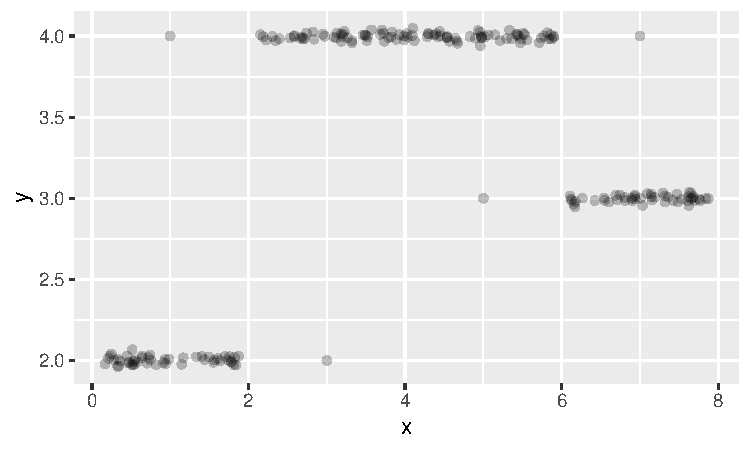
\includegraphics[width=\maxwidth]{figure/unnamed-chunk-8-1} 

}


\end{knitrout}

The above plot shows $\D = \Dset $, a data set with %$n$ observations
%data $\xv = (x^{(1)}, \dots, x^{(n)})^\top$ and $\ydat = \yvec$ for 
$n$ = 200 observations of a continuous target variable $y$ and a continuous, 
1-dimensional feature variable $\xv$. In the following, we aim at predicting 
$y$ with a machine learning model that takes $\xv$ as input.

\begin{enumerate}
  \item Assume we trained a regression tree with L1 loss $\Lxy = |y-\fx|$. 
  The training resulted in two splits of the feature $\xv$ which means that the 
  resulting estimated model is 
  \begin{align*}
  \fh (\xv) &= \sum_{m=1}^3 \hat{c}_m \I(\xv \in \hat{Q}_m)\\
   &= \hat{c}_1 \I(\xv \in (-\infty, \hat{q}_1]) + 
   \hat{c}_2 \I(\xv \in (\hat{q}_1, \hat{q}_2]) +
   \hat{c}_3 \I(\xv \in (\hat{q}_2, \infty))
  \end{align*}
  \begin{enumerate}
    \item[(i)] Estimate the two split points $\hat{q}_1$ and $\hat{q}_2$ 
    visually from the plot.
    \item[(ii)] Estimate the three predicted labels $\hat{c}_1$, 
    $\hat{c}_2$ and $\hat{c}_3$ visually from the plot.
    \item[(iii)] How would the estimated model change if we used L2 loss \\ 
    $\Lxy = 0.5 (y-\fx)^2$ instead of L1 loss? State for each split point 
    $\hat{q}_1$ and $\hat{q}_2$ and for each predicted label $\hat{c}_1$, 
    $\hat{c}_2$ and $\hat{c}_3$ 
    \begin{itemize}
      \item if it changes and
      \item if it changes, in which direction it changes
    \end{itemize}
      and explain your decision thoroughly.
  \end{enumerate}
  \item Given are two new observations $\xv_{*1} = -10$ and $\xv_{*2} = 7$. 
  State the prediction for each of the two models 
  \begin{enumerate}
    \item[(i)] regression tree
    \item[(ii)] QDA
  \end{enumerate}
  and explain how you derived the predictions.
  \item Discuss in 1-2 sentences which of the 2 models (regression tree, QDA) 
  you would prefer for modeling the data and explain your decision.
\end{enumerate}
}

\dlz
\loesung{

\begin{enumerate}
  \item \phantom{foo}
  \begin{enumerate}
    \item[(i)] $\hat{q}_1 = 2$, $\hat{q}_2 = 6$
    \item[(ii)] $\hat{c}_1 = 2$, $\hat{c}_2 = 4$, $\hat{c}_3 = 3$
    \item[(iii)] $\hat{q}_1$ and $\hat{q}_2$ would not change since including 
    more 'wrong' points is making end notes less pure, regardless of the loss. 
    (Basically no explanation needed for full point, since it does not change.)
    $\hat{c}_1$ and $\hat{c}_3$ would be higher since the L2 loss gives more 
    weight to extreme observations.
    $\hat{c}_2$ would be lower since the L2 loss gives more weight to extreme 
    observations.
  \end{enumerate}  
  \item \phantom{foo}
  \begin{enumerate}
    \item[(i)] $\hat{y}_{*1} = 2$, $\hat{y}_{*2} = 3$, 
    \item[(ii)] $\hat{z}_{*1} = 3$, since the variance of class 3 is higher, 
    the density will overshoot the density of class 1. 
    $\hat{z}_{*2} = 2$, obviously highest posterior here.
  \end{enumerate}
  \item E.g., 
  \begin{itemize}
    \item CART better than LM because I do not have to specify those indicator 
    functions manually and estimate the split points manually, CART does this 
    data driven
    \item For QDA we have to throw away information of y, this favors CART
    \item QDA predicts the middle class (3) for very extreme observations, this 
    does not seem right. However, we do not know how data behave outside the 
    bounds of x.
    \item QDA assumes gaussian distributions which is clearly not the case.
  \end{itemize}
\end{enumerate}

}

% ------------------------------------------------------------------------------

\aufgabeexam{WS2020/21}{first}{2}{

The table below shows $\D = \Dset $, a data set with 
$n$ = 5 observations of a continuous target variable $y$ and a continuous, 
1-dimensional feature variable $\xv$. In the following, we aim at predicting 
$y$ with a machine learning model that takes $\xv$ as input.

\begin{tabular}{ | c | c | c |}
\hline
ID  &  $\xv$  &  $y$  \\  \hline
1   &  1.0    &  3.1  \\
2   &  5.2    &  0.5  \\
3   &  2.7    &  1.7  \\
4   &  1.1    &  4.5  \\
5   &  1.5    &  2.7  \\
\hline
\end{tabular}

\begin{enumerate}
  \item We want to train a regression tree on the above data with the L1 loss 
  $\Lxy =|y - \fx|$. Compute the first split point $\hat{q}_1$ of the regression 
  tree.
  \item Compute the two predicted labels $\hat{c}_1$ and $\hat{c}_2$ 
  corresponding to the two resulting intervals from a).
  \item Predict the label $y$ for a new observation $\xv_* = 2$ with this 
  regression tree and explain your calculation.
\end{enumerate}

}

\dlz
\loesung{

\begin{enumerate}

  \item   

\begin{tabular}{l|r|r}
\hline
  & x & y\\
\hline
1 & 1.0 & 3.1\\
\hline
4 & 1.1 & 4.5\\
\hline
5 & 1.5 & 2.7\\
\hline
3 & 2.7 & 1.7\\
\hline
2 & 5.2 & 0.5\\
\hline
\end{tabular}


  \begin{itemize}
    \item Split $x$ in two groups using the following split points.
      \begin{itemize}
        \item $ (1)$, $(1.1,1.5,2.7,5.2)$ (splitpoint 1.05)
        \item $ (1,1.1)$, $(1.5,2.7,5.2)$ (splitpoint 1.3)
        \item $ (1,1.1,1.5)$, $(2.7,5.2)$ (splitpoint 2.1)
        \item $ (1,1.1,1.5,2.7)$, $(5.2)$ (splitpoint 4.0)
      \end{itemize}
   \item For each possible split point compute the empirical risk.
   \item Use as split point the point that splits both groups best w.r.t. 
   minimizing the empirical risk.
  \end{itemize}
  \begin{itemize}
    \item[$q = 1.05$]
      \begin{align*}
        \mathcal{R}(1, 1, 1.05) &= 0 + \sum_{i=2}^5 |y_i-median(y[2:5])|\\
        &= 0 + \sum_{i=2}^5 |y_i-2.2| \\
        &= 0 + 2.3 + 0.5 + 0.5 + 1.7\\
        &= 5
      \end{align*}
    \item[$q =  1.3$] 
      \begin{align*}
        \mathcal{R}(1, 1, 1.3) &= \sum_{i=1}^2 |y_i - median(y[1:2])|  + 
        \sum_{i=3}^5 |y_i-median(y[3:5])|\\
        &= \sum_{i=1}^2 |y_i - 3.8|  + \sum_{i=3}^5 |y_i-1.7|\\
        &= 0.7 + 0.7 + 1 + 1.2 \\
        &= 3.6
      \end{align*}
    \item[$q =  2.1$] 
      \begin{align*}
        \mathcal{R}(1, 1, 2.1) &= \sum_{i=1}^3 |y_i - median(y[1:3])|  + 
        \sum_{i=4}^5 |y_i-median(y[4:5])|\\
        &= \sum_{i=1}^3 |y_i - 3.1|  + \sum_{i=4}^5 |y_i-1.1|\\
        &= 0 + 1.4 + 0.4 + 0.6 + 0.6 \\
        &= 3
      \end{align*}
    \item[$q =  4.0$] 
      \begin{align*}
        \mathcal{R}(1, 1, 4.0) &= \sum_{i=1}^4 |y_i - median(y[1:4])|  + 0 \\
        &= \sum_{i=1}^4 |y_i - 2.9| \\
        &= 0.2 + 1.6 + 0.2 + 1.2  \\
        &= 3.2
      \end{align*}
      Minimal empirical risk is obtained by choosing the split point 
      $\hat{q} = 2.1$
  \end{itemize}
  
  \item $\hat{c}_1 = 3.1$ and $\hat{c}_2 = 1.1$

  \item Since $\xv_* = 2 < \hat{q} = 2.1$,  the observations falls in the left 
  part, i.e., the prediction is $\hat{c}_1 = 3.8$    

\end{enumerate} 

}

% ------------------------------------------------------------------------------

\aufgabeexam{WS2020/21}{second}{1}{



\begin{enumerate}
  \item We want to compare a linear regression model with a regression 
  tree. For the linear regression, we use the feature 
  variable $\xv$ without any transformations; for the regression tree, we use a 
  fully grown tree, i.e., we set the hyperparameters $cp=0$, $minsplit=1$ and 
  $minbucket=1$ in \texttt{rpart}.
  \begin{enumerate}
    \item[(i)] State the training loss of the regression tree and explain why 
    the regression tree would yield a better fit (i.e., a smaller training loss) 
    to the data than the linear regression model.
    \item[(ii)] Given the true underlying model is the cubical polynomial
    function shown with a solid line in the plot below: Which of the two models 
    (linear regression and regression tree) would extrapolate better in the 
    region $x\in (100, \infty)$? Explain your decision. 

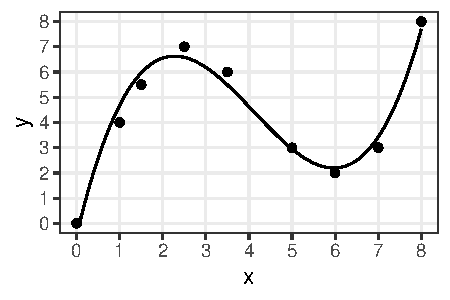
\includegraphics[width=\maxwidth]{figure/unnamed-chunk-11-1} 

  \end{enumerate}    
\end{enumerate}  

}

\newpage
\loesung{

\begin{enumerate}
  \item The training loss of the regression tree would be 0 because the fully 
  grown tree would yield a step function that goes through every point. 
  The training loss of the linear model can not be 0 since the training points 
  can not be interpolated with a straight line. 
  \item The linear model would extrapolate better because the regression tree 
  extrapolates a constant value of 8 but the true function goes further up. 
  As would go the estimated linear model.
\end{enumerate} 
}

% ------------------------------------------------------------------------------

\aufgabeexam{WS2020/21}{second}{2}{

The table below shows $\D = \Dset $, a data set with 
$n$ = 10 observations of a binary target variable \texttt{PlayTennis} and two 
binary feature variables \texttt{Temperature} and \texttt{Weather}. 
In the following, we aim at predicting \texttt{PlayTennis} with a machine 
learning model that takes \texttt{Temperature} and \texttt{Weather} as input.

\resizebox{0.88\textwidth}{!}{%
\begin{tabular}{|r|cccccccccc|}
  \hline
ID & 1 & 2 & 3 & 4 & 5 & 6 & 7 & 8 & 9 & 10 \\
  \hline
Temperature & cool & cool & cool & hot & hot & cool & hot & cool & cool & hot \\
  Weather & rain & rain & sunny & sunny & sunny & rain & rain & sunny & sunny & sunny \\
  \hline
  PlayTennis & no & no & yes & no & yes & no & yes & yes & yes & yes \\
   \hline
\end{tabular}
}
}

\begin{enumerate}
  \item We want to train a classification tree on the above data using the Brier 
  score (Gini impurity) as split criterion. Which feature will be chosen for 
  the first split? Calculate all necessary Brier scores.
\end{enumerate}

\dlz
\loesung{

\begin{enumerate}
  \item Calculate Brier score for both variables:
  \begin{itemize}
    \item \textbf{For temperature}:
    \begin{itemize}
      \item[] \textbf{N1 = hot}:
      $\hat \pi_\text{no}^\text{(hot)} = 1/4 $,
      $\hat \pi_\text{yes}^\text{(hot)} = 3/4 $,
      $Brier_\text{hot} = 2 \cdot 1/4 \cdot 3/4 = 3/8$
      \item[] \textbf{N2 = cool}:
      $\hat \pi_\text{no}^\text{(cool)} = 3/6$,
      $\hat \pi_\text{yes}^\text{(cool)} = 3/6$,
      $Brier_\text{cool} = 2 \cdot 1/2 \cdot 1/2 = 1/2 $
      \item[] Average node impurity for temperature:
      $Brier_\text{temperature} = 4/10 \cdot 3/8 + 6/10 \cdot 1/2 = .45$
    \end{itemize}
    \item \textbf{For Weather}:
    \begin{itemize}
      \item[]\textbf{N1 = sunny}:
      $\hat \pi_\text{no}^\text{(sunny)} = 1/6$,
      $\hat \pi_\text{yes}^\text{(sunny)} = 5/6 $,
      $Brier_\text{sunny} = 2 \cdot 1/6 \cdot 5/6 = 10/36$
      \item[]\textbf{N2 = rain}:
      $\hat \pi_\text{no}^\text{(rain)} = 3/4$,
      $\hat \pi_\text{yes}^\text{(rain)} = 1/4$,
      $Brier_\text{rain} = 2 \cdot 3/4 \cdot 1/4 = 3/8$
      \item[] Average node impurity for weather:
      $Brier_\text{weather} = 4/10 \cdot 3/8 + 6/10 \cdot 10/36 = .317$
    \end{itemize}
 \end{itemize}
  The split would be made on the feature \textit{weather} because the Brier 
  score of this feature is smaller.
\end{enumerate} 
}

% ------------------------------------------------------------------------------
% INSPO
% ------------------------------------------------------------------------------

\dlz
\exinspo
\end{document}
